\newpage
\section{The Enhanced Entity–Relationship (EER) Model - 04.10.22}


% Superclassi e sottoclassi
\subsection{Superclassi e sottoclassi}

L'idea è di andare a creare una \hl{gerarchia}:


\begin{figure}[H]
\centering
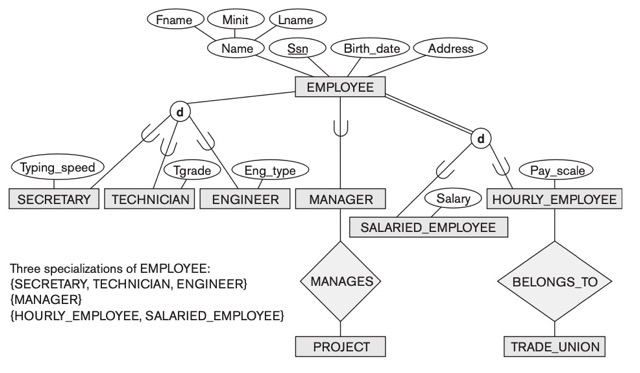
\includegraphics[scale=0.8]{gerardisg.jpeg}
\caption{Gerarchia con disjoint} 
\label{gerardisg}
\end{figure}


Per modellarlo mi chiedo quali siano le \hl{caratteristiche che hanno in comune alcune entita'}, allora tutti gli \hl{attributi in comune vanno nella superclasse}. \hl{Ogni entita' DEVE avere i suoi attributi specifici} ma non ho un attributo chiave dato che viene preso dalla superclasse.


% Graficazione superclassi e sottoclassi
\subsection{Graficazione superclassi e sottoclassi}

La graficazione avrà per:

\begin{itemize}
	\item \hl{specializzazione diretta}: si ha un segmento 
	\item \hl{gerarchia (IS-A)}: si ha un segmento con un nodo con:
		
		\begin{itemize}
			\item \textbf{d -$>$ disjoint}: NON POSSO avere un'entità che è contemporaneamente due o più sottoentità (\textbf{solo una})
			\item \textbf{o -$>$ overlap}: posso avere un'entità che è contemporaneamente due o più sottoentità (\textbf{almeno una})
			\item \textbf{U - $>$ union}: \textbf{raggruppa} entità di tipo diverso
		\end{itemize}
		
		le quali potranno avere \hl{partecipazioni totali o parziali} che indicano se la superclasse deve o meno scegliere tra le sottoclassi.
		
\end{itemize}


\begin{figure}[H]
\centering
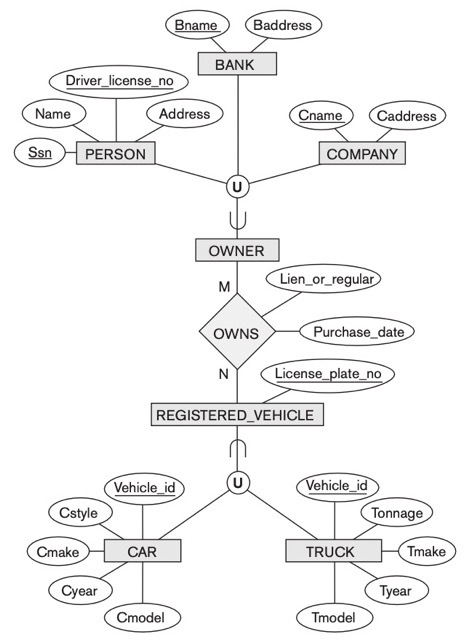
\includegraphics[scale=0.8]{union.jpeg}
\caption{Gerarchia con disjoint} 
\label{gerardisg}
\end{figure}